\documentclass[12pt]{article}
\usepackage{geometry}
\usepackage{stmaryrd}
\usepackage{imakeidx}
\geometry{left=1in,right=0.75in,top=1in,bottom=1in}

%%%%%%%%%%%%%%%%%%%%%%%%%%%%%%%%%%%%%%%%
% Replace ABCDEF in the next line with your chosen problem
% and replace 1111111 with your Team Control Number
\newcommand{\Problem}{B}
\newcommand{\Team}{2503720}
%%%%%%%%%%%%%%%%%%%%%%%%%%%%%%%%%%%%%%%%
\usepackage[backend=bibtex]{biblatex}

\usepackage{newtxtext}
\usepackage{amsmath,amssymb,amsthm}
\usepackage{newtxmath} % must come after amsXXX
\usepackage{tocloft}

% \usepackage[pdftex]{graphicx}
\usepackage{xcolor}
\usepackage{fancyhdr}
%-----数学宏包-----
\usepackage{mathrsfs,bm}
%-----draft下 label提示-----
\usepackage[notcite,notref]{showkeys}
% %-----设置超链接-----
\usepackage{url,hyperref}
\hypersetup{colorlinks=true,linkcolor=black,citecolor=black} % 去掉目录红框
%-----制作目录-----
\usepackage{imakeidx}
% 设置颜色
\usepackage{color,xcolor}
% 插入图片
\usepackage{graphicx}
\usepackage{epsfig}
%-----设置表格-----
\usepackage{tabularx,array}
\usepackage{longtable}
\usepackage{booktabs}
\usepackage{multirow}
\usepackage{multicol}
%-----调整单元格格式-----
\usepackage{makecell}
%-----操作字符串-----
\usepackage{xstring}
%-----多语种处理-----
%\usepackage[english]{babel}
%-----设置代码环境-----
\usepackage{listings}
%-----设置章节标题和目录-----
\usepackage{titling}
\usepackage{titletoc}
\usepackage{titlesec}
%-----数学公式扩展-----
\usepackage{mathtools}
%-----浮动体设置-----
\usepackage{float}
%-----书签设置-----
\usepackage{bookmark}
%-----数学宏包-----
\usepackage{amsmath,amsthm,amssymb,amsfonts}
\usepackage{mathrsfs,bm}
%-----draft下 label提示-----
\usepackage[notcite,notref]{showkeys}
% --- 算法宏包及设置 ---
\usepackage{algorithm}
\usepackage{algpseudocode}
% ---- 定义列表项的样式 -----
\usepackage{enumitem}
\setlist{nolistsep}
% --- 设置英文字体 -----
\usepackage{newtxtext}  % for text fonts
% --- 设置数学字体 -----
\usepackage{newtxmath}
% --- 直接插入 pdf 文件 ----
\usepackage{pdfpages}
\usepackage{lastpage} % 用于获取总页数
\usepackage[titletoc,title]{appendix} % 用于添加附录
\usepackage{setspace} % 用于设置行间距
% 插入图片
\usepackage{graphicx}
\usepackage{epsfig}
%-----设置表格-----
\usepackage{tabularx,array}
\usepackage{longtable}
\usepackage{booktabs}
\usepackage{multirow}
\usepackage{multicol}
%-----调整单元格格式-----
\usepackage{makecell}
%-----操作字符串-----
\usepackage{xstring}
%-----多语种处理-----
%\usepackage[english]{babel}
%-----设置代码环境-----
\usepackage{listings}
%-----设置章节标题和目录-----
\usepackage{titletoc}
\usepackage{titlesec}
%-----数学公式扩展-----
\usepackage{mathtools}
%-----浮动体设置-----
\usepackage{float}
%-----书签设置-----
\usepackage{bookmark}
\usepackage{algorithm}
\usepackage{algpseudocode}
\usepackage{setspace}
\usepackage{minted} % 用于插入代码
\renewcommand*{\baselinestretch}{1.5}
\newcommand{\upcite}[1]{\textsuperscript{\textsuperscript{\cite{#1}}}}
\definecolor{bg}{rgb}{0.95, 0.95, 0.95}
% 设置 minted 环境的全局选项
\setminted{
    linenos, % 显示行号
    frame=lines, % 添加边框
    framesep=2mm, % 设置边框与代码之间的间距
    breaklines, % 自动换行
    bgcolor=bg, % 设置背景颜色
    baselinestretch = 1.0,
    numbersep = 5pt,
    numberblanklines = false,
	tabsize = 4
}
% ----- 设置浮动体间距 ------
\setlength{\textfloatsep}{0pt}
\setlength{\floatsep}{10pt plus 3pt minus 2pt}
\setlength{\intextsep}{10pt}
\setlength{\abovecaptionskip}{2pt plus1pt minus1pt}
\setlength{\belowcaptionskip}{3pt plus1pt minus2pt}

% ----- 设置公式间距为零 ------
\AtBeginDocument{
	\setlength{\abovedisplayskip}{4pt plus1pt minus1pt}
	\setlength{\belowdisplayskip}{4pt plus1pt minus1pt}
	\setlength{\abovedisplayshortskip}{2pt}
	\setlength{\belowdisplayshortskip}{2pt}
	\setlength{\arraycolsep}{2pt}   % array中列之间空白长度
}
% ---- 定义列表项的样式 -----
\usepackage{enumitem}
\setlist{nolistsep}
% \setlength{\itemsep}{3pt plus1pt minus2pt}

% --- 设置英文字体 -----
% \usepackage{newtxtext}  % for text fonts
\usepackage{fontspec}


% --- 自定义命令 -----
\newcommand{\CC}{\ensuremath{\mathbb{C}}}
\newcommand{\RR}{\ensuremath{\mathbb{R}}}
\newcommand{\A}{\mathcal{A}}
\newcommand{\ii}{\bm{\mathrm{i}}\,}  % 虚部
\newcommand{\md}{\mathrm{d}\,}
\newcommand{\bA}{\boldsymbol{A}}
\newcommand{\red}[1]{\textcolor{red}{#1}}


\lhead{Team \Team}
\rhead{}
\cfoot{}

\newtheorem{theorem}{Theorem}
\newtheorem{corollary}[theorem]{Corollary}
\newtheorem{lemma}[theorem]{Lemma}
\newtheorem{definition}{Definition}

% 定义 summary 环境
\newenvironment{summary}
  {\begin{center}\bfseries Summary\end{center}\normalfont}

% 重新定义目录标题并居中显示
\renewcommand{\contentsname}{\centering Contents}

% 设置页眉
\pagestyle{fancy}
\fancyhf{}
\fancyhead[L]{Team \# 2503720}
\fancyhead[R]{Page \thepage\ of \pageref{LastPage}}
%%%%%%%%%%%%%%%%%%%%%%%%%%%%%%%%




\begin{document}

\onehalfspacing

\thispagestyle{empty}

\vspace*{-16ex}
\centerline{\begin{tabular}{*3{c}}
	\parbox[t]{0.3\linewidth}{\begin{center}\textbf{Problem Chosen}\\ \Large \textcolor{red}{\Problem}\end{center}}
	& \parbox[t]{0.3\linewidth}{\begin{center}\textbf{2025\\ MCM / ICM\\ Summary Sheet}\end{center}}
	& \parbox[t]{0.3\linewidth}{\begin{center}\textbf{Team Control Number}\\ \Large \textcolor{red}{\Team}\end{center}}	\\
	\bottomrule
\end{tabular}}

\begin{center}
    \Large{\textbf{This is the title}}
\end{center}

\begin{summary}
    Here is the abstract of our paper. Here is a test.
\end{summary}
    

\clearpage



%%%%%%%%%%%%%目录%%%%%%%%%%%%%%

\tableofcontents

%%%%%%%%%%%%%%%%%%%%%%%%%%%%%
\clearpage
\pagestyle{fancy}

%%%%%%%%%%%%%%%%%%%%%%%%%%%%%%

\section{Introduction}

\subsection{Background}

Juneau, the capital city of Alaska, seamlessly combines 
breathtaking natural beauty with a rich cultural heritage. 
Nestled in the southeastern part of the state, this unique city 
is accessible only by air or sea, giving it an island-like allure 
despite being located on the mainland. Home to approximately 30,000 
residents, Juneau welcomes over a million tourists annually—a number 
that continues to grow each year. While tourism has significantly 
boosted the city’s economy, it has also brought challenges, such 
as receding glaciers, increasingly crowded streets, and rising 
carbon emissions. To ensure its long-term prosperity, Juneau 
must embrace a \textbf{sustainable tourism strategy} that balances growth 
with the preservation of its natural and cultural treasures, which will be
presented in the following sections.


\subsection{Restatement and Analyses of the Problem}

We need to complete the following tasks based on the given background
and our collected data.

\begin{itemize}
    \item \textbf{Task 1: Develop a model to quantify the tourism industry in Juneau and analyse the model.}
    \begin{itemize}
        \item The model is required to qualitatively and quantitatively analyze the factors that affect the tourism industry in Juneau, including the economy, society, and environment. 
        \item The model should be able to predict the number of tourists in the next few years and provide insights into the development of the tourism industry in Juneau.
        \item A sensitivity anslysis should be conducted to evaluate the robustness of the model.
    \end{itemize}
    \item \textbf{Task 2: Test the model's adaptability and migration capability in Sitka, Alaska.}
    \\Based on the model developed in Task 1, we need to adapt the model to the city of Sitka, Alaska, and test its adaptability and migration capability.
    \item \textbf{Task 3: Propose a sustainable tourism strategy for Juneau.}
    \\Based on the model developed in Task 1, we need to propose a sustainable tourism strategy for Juneau that balances economic growth with environmental and social sustainability.
\end{itemize}

It can be noted that task 1 serves as the foundation for Task 2 and Task 3, 
while Task 2 provides a practical application of the model developed in Task 1. 
Task 3 aims to address the challenges and opportunities identified in Task 1 and Task 2, 
providing a comprehensive and sustainable solution for the tourism industry in Juneau.

Questions can be asked to further clarify the problem:
How to quantify the tourism industry in Juneau? Which factors should be 
considered in the model and what methods should be used? After developing 
the model, how can we adapt it to another city? What suggestions and 
strategies can be proposed to promote the sustainable development of the
tourism industry in Juneau?

In summary, we should effectively build a model that can quantify the tourism
industry in Juneau, adapt the model to another city, and propose a sustainable
tourism strategy for Juneau.


\subsection{Overview of Our Work}

On the basis of the above analyses we carried out out work and the 
working framework is shown below.

\begin{figure}[H]
    \centering
    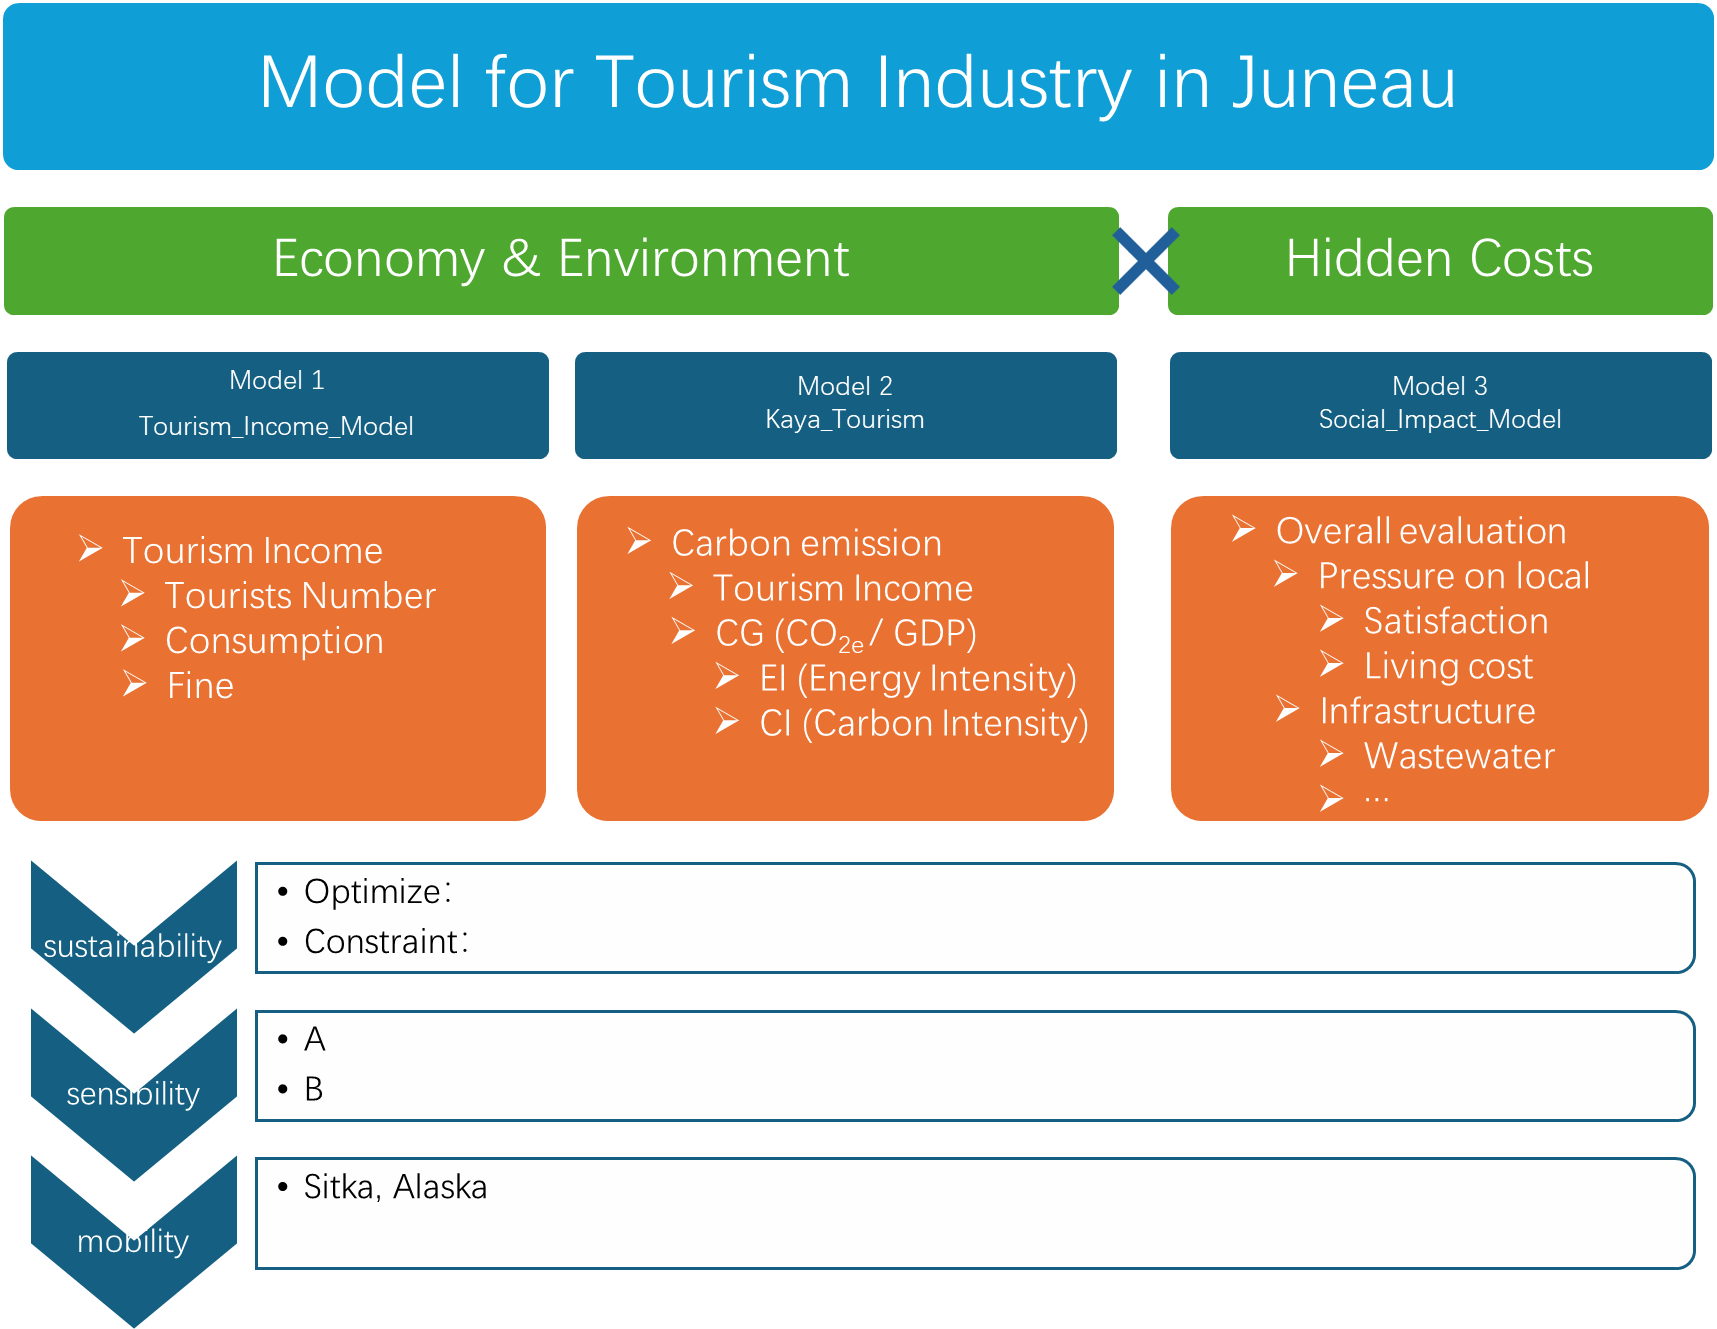
\includegraphics[width=0.8\textwidth]{Framework.png} % 插入图片
    \caption{Our Work Overview Schematic Diagram}
\end{figure}



\section{Preparations of the Models}

\subsection{Assumptions}

\subsection{Notations}

The primary notations used in this paper are listed in Table 1.

\begin{table}[!htbp]
  \begin{center}
  \caption{Notations}
  \begin{tabular}{cl}
    \toprule
    \multicolumn{1}{m{3cm}}{\centering Symbol}
    &\multicolumn{1}{m{8cm}}{\centering Definition}\\
    \midrule
    $A$&the first one\\
    $b$&the second one\\
    $\alpha$ &the last one\\
    \bottomrule
  \end{tabular}
  \end{center}
  \end{table}

\subsection{Assumptions}

The following reasonable assumptions are made to reasonably simplify the model:

\begin{itemize}
  \item Government policies (such as taxes, subsidies, regulations, etc.) remain unchanged during the period of the model.
  \item No major event compromising or promoting the tourism industry will occur during the period of our model.
  \item Consumer behavior, consumer preferences, or market demand are assumed to remain unchanged.
\end{itemize}


\section{Assumptions and Notations}


\clearpage


\section{Task 1: Model for Tourism Industry in Juneau}

\subsection{Introduction}


In this section we need to select factors to quantify and track the tourism industry in Juneau. 
It is impossible and unnecessary to consider all the factors that may affect the 
tourism industry, only those that are relevant to the problem need to be considered.
Drawing on the idea of the divide-and-conquer algorithm, we first divide the factors 
into three categories: economy, society and environment. 


\begin{equation}
    \mathbb{T}\text { Output }=\alpha \cdot \text { Economy }-\beta \cdot \text { Society }-\gamma \cdot \text { Environment }
\end{equation}

Our goal is to maximize the economy income, minimize the social cost and environmental impact,
where parameters $\alpha$, $\beta$ and $\gamma$ denote how much importance we attach to each category.
Intuitively, the goal aforementioned is equivalent to maximizing the output.

Each category is further divided into several minor factors such as local population, 
number of tourists to extrapolate a mathematical model fitting the circumstances in Juneau,
which will be discussed in the following sections.





\subsection{Economy}

In this section we consider the actions that will contribute to the income of the tourism industry in Juneau, which are
tourists' consumption, tax income and fines.

\subsubsection{Tourists' Consumption}


\subsection{Society}

Societal factors such as infrastructure, price of housing products, and the mental
loss due to the overcrowding and rowdy tourists all account for the social cost of the tourism industry.

\subsection{Environment}

According to the official website of Juneau, its tourism industry is 
mainly comprised of glacier tours, whale watching, rainforest tours and others.
We assume each of these activities accounts for a certain percentage of the total environmental impact,
denoted as $v_1$, $v_2$, $v_3$ and $v_4$ respectively. Due to the receding of glaciers,
our goal is to lower the percentage of glacier tours and increase the percentage of other activities.

The main factors that affect the environment are carbon emissions and human disturbance, which will be discussed as follows.

\clearpage


\section{Task 2}



\section{Task 3}

% \begin{appendices}
%     \section{Further on \LaTeX}
%     \section{Program Codes}
%     \begin{minted}{cpp}
%   #include <iostream>
%   using namespace std;
%   int main() {
%       cout << "Hello, World!" << endl;
%       return 0;
%   }
%     \end{minted}
%   \end{appendices}


\addcontentsline{toc}{section}{References}

\begin{thebibliography}{99}
  \bibitem{mcdowell2016} McDowell Group. (2016). \textit{ Juneau Visitor Profile and Economic Impact Study}. 
  \bibitem{southeast2023} Southeast Conference. (2023).  \textit{Juneau Tourism Survey 2023}. 
  \bibitem{juneau2016} City and Borough of Juneau. (2016).  \textit{Juneau’s Visitor Industry: Positive Economic Benefits for Our Community}. 
  \bibitem{jedc2024} Juneau Economic Development Council (JEDC). (2024).  \textit{Juneau SEAK Economic Indicators and Outlook Report}. 
  \bibitem{juneau2021} City and Borough of Juneau. (2021).  \textit{Juneau Tourism Survey 2021}. 
  \bibitem{juneau2022} City and Borough of Juneau. (2022).  \textit{Juneau Tourism Survey 2022}. 
  \bibitem{juneau2023} City and Borough of Juneau. (2023).  \textit{Juneau Tourism Survey 2023}. 
  \bibitem{circulator2024} City and Borough of Juneau. (2024).  \textit{Juneau Visitor Circulator Study: Final Report}. 
  \bibitem{budget2016} City and Borough of Juneau Assembly. (2016).  \textit{Biennial Budget Fiscal Year 2016: Year 2 of the FY15/FY16 Biennial Budget}. 
  \bibitem{budget2018} City and Borough of Juneau. (2018).  \textit{Biennial Budget Adopted Fiscal Year 2018: Year 2 of the FY17/18 Biennial Budget}. 
  \bibitem{budget2020} City and Borough of Juneau. (2020).  \textit{Biennial Budget Adopted Fiscal Year 2020: Year 2 of the FY19/20 Biennial Budget}. 
  \bibitem{budget2022} City and Borough of Juneau. (2022).  \textit{Biennial Budget Adopted Fiscal Year 2022: Year 2 of the FY21/22 Biennial Budget}. 
  \bibitem{budget2024} City and Borough of Juneau. (2024).  \textit{Biennial Budget Adopted Fiscal Year 2024: Year 2 of the FY23/24 Biennial Budget}. 
  \bibitem{alaskaInventory}Alaska Department of Environmental Conservation Division of Air Quality. (2023). \textit{Alaska Greenhouse Gas Emissions Inventory}.
\end{thebibliography}

\end{document}
